\documentclass[final, english, english, a4paper, 12pt, numbers=noenddot, % Bei Änderung der Sprache 2 x kompilieren!
% tudscr spezifische Einstellungen
cd=false,
cdfont=false,cdfont=nohead,
cdmath=false,
cdhead=false,
cdfoot=true,
cdcover=monochrome,
cdgeometry=asymmetric,
declaration=heading,
declaration=notoc,
abstract=heading,
]{tudscrreprt}

%################ Hilfreiche Pakete laden #######################

%################ Hilfreiche Pakete laden #######################

\usepackage{settings/tudbwlimPackages}
\usepackage{settings/tudbwlimStyle}
\usepackage{scrhack}
\usepackage{microtype}
\usepackage{tikz,pgfplots}
\pgfplotsset{compat=newest}
\usepackage[chapter]{algorithm} % Falls das Paket floatrow geladen wird, muss dieses Paket danach geladen werden.
\iflanguage{english}{\floatname{algorithm}{Algorithm}\renewcommand{\listalgorithmname}{List of Algorithms}}{\floatname{algorithm}{Algorithmus}\renewcommand{\listalgorithmname}{Algorithmenverzeichnis}} % Algorithm-Umgebung an die verwendete Sprache anpassen
\usepackage{comment}
\usepackage{subcaption}
\usepackage{caption}
\usetikzlibrary{positioning}
\usetikzlibrary{mindmap}
\usepackage{graphicx}
\usepackage{float}
\usepackage{longtable}
\usepackage{xparse} % for \NewDocumentCommand
\usepackage{multirow}
\usepackage{array}
\usepackage{makecell}
\usepackage[justification=centering]{caption} % Für die Zentrierung der Bildunterschrift

%################ Notwendige Pakete laden #######################


\usepackage[bibencoding=auto,citestyle=authoryear-ibid,bibstyle=authoryear,maxcitenames=3,maxbibnames=10, backend = biber]{biblatex}% Vergessen Sie nicht in den Optionen das Bibliographieprogramm auf "biber" umzustellen! Um die Vorlage mit BibTeX nutzen zu können, muss die Option "backend=bibtex" übergeben werden. Es ist jedoch biber zu empfehlen, beachten Sie dazu die Hinweise der biblatex-Paketdokumentation im Abschnitt 3.15 "Using the fallback BibtTeX backend".
\usepackage{settings/BiblatexSetup}

\AfterPackage*{biblatex}%
{
    \RequirePackage[breaklinks=true, colorlinks=true, linktoc=section, linkcolor=blue, citecolor=black, hidelinks]{hyperref}
    % Da hyperref allerhand Veränderungen an vielen Standardbefehlen vornimmt, sollte dieses als letztes in der Präambel eingebunden werden. Nur Pakete, bei denen in der Dokumentation explizit darauf hingewiesen wird, dass diese nach hyperref zu laden sind, sollten auch danach folgen.
    \hypersetup{pdfprintscaling=None} % gleiches Verhalten, auch ohne hyperref, liefert: \pdfcatalog{/ViewerPreferences<</PrintScaling/None>>}
    \usepackage{footnote} % https://tex.stackexchange.com/questions/207192/footcite-in-float-caption
    \makesavenoteenv{figure}
    \makesavenoteenv{table}
    \makesavenoteenv{algorithm}
}


\AfterPackage*{hyperref}
{
    \RequirePackage[automake,acronym,symbols,nomain,translate=babel]{glossaries}
    \usepackage{settings/GlossariesSetup}
}
%############## Own commands #####################´
\newcommand{\parbreak}{\vspace{\baselineskip}\noindent}
\newcommand{\gendreauDataSet}{Gendreau (2006)}
\newcommand{\mouraDataSet}{Moura (2009)}
\newcommand{\ceschiaDataSet}{Ceschia (2013)}
\newcommand{\krebsADataSet}{Krebs (2021a)}
\newcommand{\krebsBDataSet}{Krebs (2021b)}
\newcommand{\gendreauDataSetText}{\gendreauDataSet\ }
\newcommand{\mouraDataSetText}{\mouraDataSet\ }
\newcommand{\ceschiaDataSetText}{\ceschiaDataSet\ }
\newcommand{\krebsADataSetText}{\krebsADataSet\ }
\newcommand{\krebsBDataSetText}{\krebsBDataSet\ }

%############## Ideas for packages #####################´
% Folgende auskommentierte Pakete sind als Vorschläge zu verstehen. Für Funktionsweise und Anwendungsfälle wird auf das Benutzerhandbuch "tudscr.pdf" (http://mirrors.ctan.org/macros/latex/contrib/tudscr/doc/tudscr.pdf) oder auf die entsprechende CTAN Dokumentation verwiesen.
%\usepackage{listings} %For Visualization of programming source code 
%\lstset{%
%	inputencoding=utf8,extendedchars=true,
%	literate=%
%	{ä}{{\"a}}1 {ö}{{\"o}}1 {ü}{{\"u}}1
%	{Ä}{{\"A}}1 {Ö}{{\"O}}1 {Ü}{{\"U}}1
%	{~}{{\textasciitilde}}1 {ß}{{\ss}}1
%	}

%\usepackage{calc} % Can be used to calculate inline distances in .tex files

%################ Sonstige Einstellungen/Befehle #####################
\onehalfspacing

%################ Abkürzungen #######################
\glsenableentrycount % aktiviert \cgls, \cglspl, \cGls, \cGlspl, siehe https://tex.stackexchange.com/questions/98494/glossaries-dont-print-single-occurences/230664#230664

% Abkürzungen, die im Abkürzungsverzeichnis auftauchen und automatisch durch das glossaries-Paket sortiert werden
\newacronym[description={Container loading problem}]{CLP}{CLP}{container loading problem}
\newacronym[description={Vehicle routing problem}]{VRP}{VRP}{vehicle routing problem}
\newacronym[description={Capacitated vehicle routing problem}]{CVRP}{CVRP}{capacitated vehicle routing problem}
\newacronym[description={Bin packing problem}]{BPP}{BPP}{bin packing problem}
\newacronym[description={Last-in-first-out}]{LIFO}{LIFO}{last-in-first-out}
\newacronym[description={Cutting and packing}]{CaP}{C\&P}{cutting and packing}
\newacronym[description={Constraint programming}]{CP}{CP}{constraint programming}
\newacronym[description={Mixed-integer programming}]{MIP}{MIP}{mixed-integer programming}
\newacronym[description={Genetic algorithm}]{GA}{GA}{genetic algorithm}
\newacronym[description={Tabu search}]{TS}{TS}{tabu search}
\newacronym[description={Simulated annealing}]{SA}{SA}{simulated annealing}
\newacronym[description={Greedy randomized adaptive search procedure}]{GRASP}{GRASP}{greedy randomized adaptive search procedure}
\newacronym[description={Variable neighborhood search}]{VNS}{VNS}{variable neighborhood search}
\newacronym[description={Pallet loading problem}]{PLP}{PLP}{pallet loading problem}
\newacronym[description={Machine learning}]{ML}{ML}{machine learning}
\newacronym[description={Artificial neural network}]{ANN}{ANN}{artificial neural network}
%\newacronym[description={Support vector machine}]{SVM}{SVM}{support vector machine}
\newacronym[description={Logistic regression}]{LR}{LR}{logistic regression}
\newacronym[description={Two-dimensional loading capacitated vehicle routing problem}]{2L-CVRP}{2L--CVRP}{two-dimensional loading capacitated vehicle routing problem}
\newacronym[description={Three-dimensional loading capacitated vehicle routing problem}]{3L-CVRP}{3L--CVRP}{three-dimensional loading capacitated vehicle routing problem}
\newacronym[description={Three-dimensional loading vehicle routing problem with time windows}]{3L-VRPTW}{3L--VRPTW}{three-dimensional loading vehicle routing problem with time windows}
\newacronym[description={Time windows}]{TW}{TW}{time windows}
%\newacronym[description={Lower bound}]{LB}{LB}{lower bound}
\newacronym[description={Upper bound}]{UB}{UB}{upper bound}
\newacronym[description={Manual last-in-first-out}]{MLIFO}{MLIFO}{manual last-in-first-out}
\newacronym[description={Load-bearing strength}]{LBS}{LBS}{load-bearing strength}


% Abkürzungen, die nicht im Abkürzungsverzeichnis aufgeführt werden
%\newabbreviation{zB}{z.\,B.}{zum Beispiel}

% Do i need this? 
\glsaddall[types=abbreviation]

% Symbole die im Symbolverzeichniss erscheinen sollen
% Mit "F5" kompilieren oder "Tools -> Befehle -> makeglossaries" (F9) starten, um das Symbolverzeichnis zu aktualisieren
% \newsymb{<sort by>}{<name>}{<symbol>}{<unit>}
%
\begin{comment}
\newsymb{E}{Erwartungswert}{\mathbb{E}\left(\cdot\right)}{}
\newsymb{P}{Wahrscheinlichkeitsmaß}{\mathbb{P}\left(\cdot\right)}{}
\newsymb{V}{Varianz}{\mathbb{V}\left(\cdot\right)}{}
\newsymb{X}{Zufallsvariable}{X}{}
%
% Oder so verwenden und im Fließtext dann mit $\ExpValue$ arbeiten:
%\newcommand{\ExpValue}{\mathbb{E}\left(\cdot\right)}
%\newsymb{E}{Erwartungswert}{\ExpValue}{}
%
\glsaddall[types={symbols}] % Alle Symbole werden dem Symbolverzeichnis hinzugefügt
\end{comment}

%################ Bibliographie laden #######################
\addbibresource{./Forschungsseminar_References.bib} % Pfad/Name der .bib-Datei

%################ Ende Präambel #######################
\pagenumbering{Roman}

\begin{document}
%################ Aufruf Deckblatt #######################
% mögliche Optionen, für weitere Informationen, siehe S. 23 des Benutzerhandbuchs des tudscr-Paket (http://mirrors.ctan.org/macros/latex/contrib/tudscr/doc/tudscr.pdf):

%%%%%%%%%%%%%%%%%%%%%%%%%%%%%%%%%%%%%
%\thesis{\diplomathesisname}		% Diplomarbeit/Diploma-Thesis
%\graduation[Dipl.-Kffr.]{Diplom-Kauffrau} % [Dipl.-Kfm.]{Diplom-Kaufmann}
%
%\thesis{\masterthesisname}			% Master-Arbeit/Master Thesis
%\graduation[M.Sc.]{Master of Science}
%
%\thesis{\bachelorthesisname}		% Bachelor-Arbeit/Bachelor Thesis
%\graduation[B.Sc.]{Bachelor of Science}

\renewcommand{\seminarCategoryText}{As part of the Industrial Management research seminar}
\renewcommand{\seminarpapername}{Exposé}
\newsavebox\thesisbox
\savebox\thesisbox{\normalfont\large\sffamily \parbox{\textwidth}{\vspace{6pt} \raggedright \seminarCategoryText}}
% https://github.com/tud-cd/tudscr/issues/85 %
%
\thesis{\seminarpapername \seminarCategory{\\\usebox\thesisbox}}		% Seminararbeit/Seminar Paper
%%%%%%%%%%%%%%%%%%%%%%%%%%%%%%%%%%%%%

\title{Feasibility prediction for the container loading problem}
%\subtitle{Optionaler Unter-/Zusatztitel}
\author{%
	Maximilian Hubmann
	\matriculationnumber{4805234}
	\dateofbirth{21.03.2000}
	\placeofbirth{Nürnberg}
	\course{Wirtschaftsingenieurwesen, 9. FS}
}
\date[]{\today}
\supervisor{Dipl.-Wi.-Ing. Florian Linß}
\professor{Prof. Dr. Udo Buscher}

\setcounter{page}{1}

%%% IM 
\headlogo{./pictures/IM-Logo}
\faculty{Faculty of business and economics}
\chair{Chair of Business Administration, in particular Industrial Management}
\maketitle[cdtitle=true, cdfont=false]

%################ Abstract ######################
%\begin{abstract}
%Das ist ja maal so cool, dass ich ich einfahc hier einen Tsext schreiben kann
%\end{abstract}

%%% Danksagung
%\danke{Danksagung}{Text}

%####################### Verzeichnisse ################%
%\microtypesetup{protrusion=false}
% Inhaltsverzeichnis
\tableofcontents

% Abbildungsverzeichnis (falls nichts benötigt, einfach als Kommentar setzen)
\listoffigures
\addcontentsline{toc}{chapter}{\listfigurename}

% Tabellenverzeichnis (falls nichts benötigt, einfach als Kommentar setzen)
\listoftables
\addcontentsline{toc}{chapter}{\listtablename}

% Algorithmenverzeichnis (falls nichts benötigt, einfach als Kommentar setzen)
%\listofalgorithms
%\addcontentsline{toc}{chapter}{\listalgorithmname}

\microtypesetup{protrusion=true}

%Abkürzungsverzeichnis (falls nichts benötigt, einfach als Blockkommentar setzen)
\printacronyms[style=bwlimsuper]
\addcontentsline{toc}{chapter}{\acronymname}

% Symbolverzeichnis (falls nichts benötigt, einfach als Blockkommentar setzen)
% \printsymbols[style=symblong, title=\listsymbolname]
% \addcontentsline{toc}{chapter}{\listsymbolname}



%############### Einstellungen für Fließtext setzen ####################
\clearpage
\setcounter{page}{1}\pagenumbering{arabic}

%####################### Fließtext ####################

\chapter{Introduction}
\label{sec:introduction}
Efficiently arranging items of varying shapes and sizes within a container is a fundamental challenge
in logistics and supply chain management. This \gls{CLP} arises in numerous real-world contexts,
such as loading cargo onto ships, trucks, and aircraft, as well as optimizing warehouse storage and
packing of smaller goods into pallets or cardboard boxes\footcite[cf.][p.1]{bortfeldt_constraints_2013}.

\parbreak

The \gls{CLP}, particularly in its multi-dimensional variants, is classified as an NP-hard problem.
Real-world constraints—such as orientation rules, stability requirements, and load-bearing
limitations—add further complexity to the problem\footcite[cf.][p.377-378]{bischoff_issues_1995},
and are elaborated in Chapter~\ref{sec:clp_definition}. As such, exact algorithms are limited to
small instances, and research has focused on heuristic approaches,
as discussed in Chapter~\ref{sec:classical_solution_approaches}.

\parbreak

In complex scenarios, recent research demonstrates that \gls{ML} models can help to reduce the computation
time finding good solutions. Especially classifiers were succesfully integrated in existing algorithms
and are presenred in Chapter~\ref{sec:motivation_feasibility_prediction} \footcite[cf.][]{zhang_learning-based_2022}.
A suitable use case for using a classifier is the \gls{3L-CVRP}, where single tours of the \gls{VRP}
represent a \gls{CLP} with cuboids themselves and numerous tours need to be comutational expensively checked for feasibility
\footcite[cf.][p. 1]{tamke_branch-and-cut_2024}. However, current research of classifiers of tours
rely on simplified assumptions that do not fully capture practical constraints. Therefore, suitable \gls{3L-CVRP}
datasets are compared in Chapter~\ref{sec:dataset_selection} and a suitable dataset is selected to
lay the foundation for training a classifier. Finally, this paper aims to bridge this gap by examining constraint
datasets relevant to the \gls{3L-CVRP}, thereby enabling more realistic feasibility predictions for
future work, which is depicted in Chapter~\ref{sec:conclusion}.


\chapter{The Container Loading Problem}
\label{sec:clp_definition}

The placement and assignment of items to larger, mostly rectangular
containers, is a well known problem in logistics and operations research, as the
potential of cost savings and efficiency gains is substantial by reducing the number
of needed containers or by fulfilling customer needs \footcite[cf.][p.1]{bortfeldt_constraints_2013}.
\gls{CLP} problems are differentiated by \cite{bortfeldt_constraints_2013} in \textit{input minimization},
where the number of needed containers is minimized, and \textit{output maximization} problems,
where the value of the associated items is maximized. So, is the \gls{BPP} belonging
to \textit{input minimization} problems, and the \gls{KP} to \textit{output maximization}.

Apart from the expected outcome of the optimization, the characterics of the items
and containers is relevant for the problem definition. Items can be either homogenous or heterogenous,
where homogenous items are identical in size and shape, and heterogenous items are
different in size and shape. The container is usually defined as a gls{3D} space
with a fixed size and shape, where the items have to be placed in.
Other - non rectangular - shapes are scarcely considered in the literature, as the practical relevance is
limited \footcite[cf.][p.1-2]{bortfeldt_constraints_2013}. Multiple containers, with homogeneous
or heterogenous size,  are used, whenever the volume and weight of the items requires it.
A possible placement of cargo into a container can be seen in Figure \ref{fig:solution-visualization}.

\begin{figure}[ht]
    \centering
    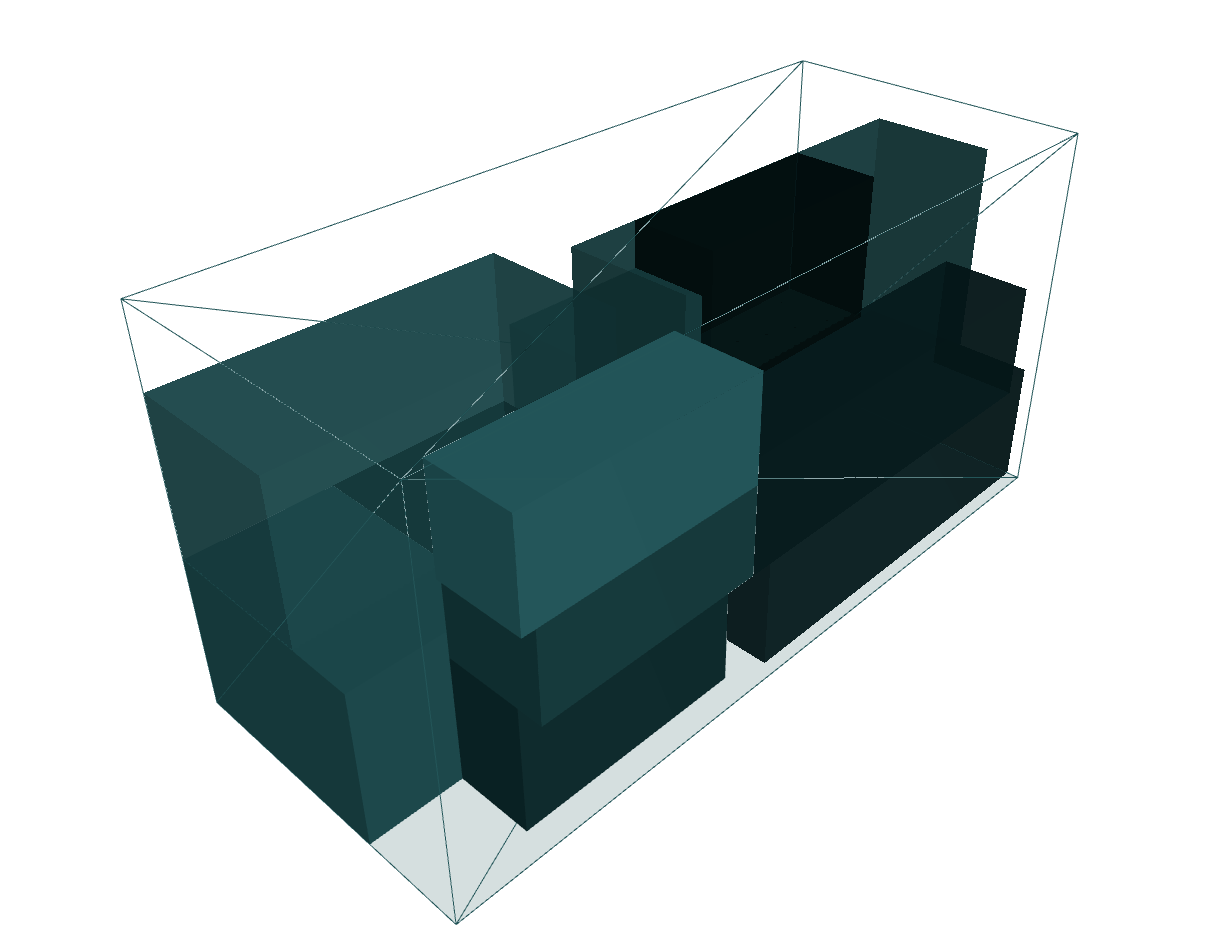
\includegraphics[width=7cm]{pictures/3l_cvrp_example.png}
    \caption[Visualized 3D packing with packing constraints]{Visualized 3D packing with packing constraints\footnotemark}.
    \footnotetext{Visualization from \cite{tamke_branch-and-cut_2024}}
    \label{fig:solution-visualization}
\end{figure}

According to \cite{bischoff_issues_1995}, the mere placement of items is insufficient
if practical requirements are not fulfilled. Building on this insight,
\cite{bortfeldt_constraints_2013} systematically categorized all constraints relevant
to the \gls{CLP} into five groups. They also distinguish between hard and soft constraints,
where hard constraints must be strictly satisfied, while soft constraints may be violated
to some extent, depending on the implementation context.
It should also be noted that, by referring to the standard problems of \gls{CaP},
certain assumptions are implicitly adopted. For instance, in line with common
practice in the literature only orthogonal placements are allowed, so box surfaces must be
aligned parallel to the container floor and walls \footcite[cf.][p.2]{bortfeldt_constraints_2013}

\subsubsection{Container related constraints}
These constraints summarize all physical barriers of the container. The \textbf{load capacity} limits the aggregated
mass of all items in the container. The distribution of the weight (\textbf{load balance})
plays also an important role for safety reasons, as the cargo must not move during the transport and the container
must not tip over and is defined by the maximum weight difference between the left and right half of the container.
In the special case of trucks, uneven \textbf{axle weight} distribution can cause severe
crash consequences and need to be avoided by loading the cargo axle-friendly \footcite[cf.][pp. 849--850]{krebs_advanced_2021}.

\subsubsection{Item related constraints}
Item related constraints define the properties of the item, which are relevant
for the packing. When the container capacity is limited (\textit{output maximization}),
the \textbf{loading priority} constraint can define the priority among possible
item candidates. The orientation constraint restricts how an item can be rotated.
Several rotation types exist, each defined by the axis around which the item can rotate.
The most common is the \textbf{z-rotation}, where rotation is only allowed around the vertical (z) axis.
When 3D packing is considered, the \textbf{fragility} constraint
is relevant for defining which items can be stacked on top of each other. Items are
differentiated between \textit{fragile} and \textit{non-fragile}, stating
that non-fragile items can only be stacked on non-fragile items, Figure \ref{fig:stacking_comparison} showcases
this definition. A more sophisticated approach is the calculation of the
\textit{load-bearing strength}(\textbf{LB Strength}) of each box, stating how much pressure the box
can tolerate \footcite[cf.][pp. 847--848]{krebs_advanced_2021}.

\begin{figure}[htbp]
    \centering
    % First TikZ picture
    \begin{subfigure}[b]{0.45\textwidth}
        \centering
        \begin{tikzpicture}
            % Draw the container
            \draw[thick] (0,0) rectangle (5,3);

            % Draw the three items inside
            \draw[fill=blue!20] (3,0) rectangle (5,0.75);
            \node at (4, 0.5) {};

            \draw[fill=green!20] (3,0.75) rectangle (5,1.5);
            \node at (4, 1.125) {Fragile};

            \draw[fill=green!20] (3,1.5) rectangle (5, 2.25);
            \node at (4, 1.875) {Fragile};

        \end{tikzpicture}
        \caption{Feasible stacking of items}
    \end{subfigure}
    \hfill
    % Second TikZ picture
    \begin{subfigure}[b]{0.45\textwidth}
        \centering
        \begin{tikzpicture}
            \draw[thick] (0,0) rectangle (5,3);

            % Draw the three items inside
            \draw[fill=blue!20] (3,0) rectangle (5,0.75);
            \node at (4, 0.5) {};

            \draw[fill=green!20] (3,0.75) rectangle (5,1.5);
            \node at (4, 1.125) {Fragile};

            \draw[fill=blue!20] (3,1.5) rectangle (5, 2.25);
            \node at (4, 1.875) {};
        \end{tikzpicture}
        \caption{Infeasible stacking of items}
    \end{subfigure}
    \caption[Visualization fragile stacking]{Comparison fragile stacking \footnotemark}
    \footnotetext{Own figure}
    \label{fig:stacking_comparison}
\end{figure}


\subsubsection{Cargo-Related Constraints}
In contrast to item-related constraints, cargo-related constraints apply to
the entire cargo or to specific subsets of it. The \textbf{complete-shipment} constraint
requires that all items within a shipment must either be loaded into the same
container or be left behind entirely. This constraint is especially important
when container capacity is limited (\textit{output maximization}) and items
cannot be split. The \textbf{allocation constraint} serves a similar purpose.
It includes the \textbf{connectivity constraint}, which mandates that
certain items must be loaded into the same container, and the
\textbf{separation constraint}, which requires specific items to
be distributed across different containers. For example, kitchen
shipments—comprising multiple packages-should be delivered together
to enable efficient installation. Conversely, items such as perfume and fresh
vegetables should be shipped separately due to incompatibility.

\subsubsection{Positioning constraints}

Positioning constraints in container loading determine where items can be placed,
either in absolute (specific location) or relative to other items.
The absolute positioning constraints specify that certain items
must (or must not) be placed in specific areas of the container. These are
typically based on item characteristics such as size, weight, or
content (e.g., bulky or hazardous items placed near the container door for accessibility) or
exist in general for all item types, as the \textbf{geometry} and
\textbf{orthogonality} constraints. These constraints define that items are not allowed to overlap
and must be placed orhogonally to the container walls respectively.
Relative positioning constraints govern how items are arranged in
relation to each other. Either close to each other as \textit{group} or
\textit{separate} from each other. This differentiation is similar to the
\textit{allocation constraint} of the cargo-related constraints, but considers
only one container.
The \textbf{multi-drop constraints} combine
absolute and relative positioning requirements when items are destined for
different delivery locations. These constraints aim to minimize reloading
efforts by grouping items by delivery destination, by arranging item groups
in accordance with the delivery sequence and/or by applying a
\textbf{\gls{LIFO}} or \textbf{sequential loading policy}
to ensure efficient unloading without moving unrelated items. Adaptions of the \gls{LIFO} constraint,
consider either, that the items can be unpacked manually (\textbf{\gls{MLIFO}}) or can be unloaded generally
with a maximum distance to the unloading point (\textbf{reachability constraint}). These
types of positioning constraints are widely discussed in the iterature due
to their practical relevance in real-world logistics operations.

\subsubsection{Load-related constraints}

The \textbf{stability constraint} is defined as one of the most critical constraints
in the \gls{CLP}, as it directly impacts
the safety of both the cargo and the personnel involved. First, a distinction
must be made between \textit{horizontal} and \textit{vertical} stability.
Horizontal stability is achieved when items are securely connected to the
container walls or to other items, preventing lateral movement. Vertical
stability, on the other hand, is defined in various ways throughout the
literature. One common approach evaluates the supporting area — the portion
of an item's base that rests on the surface below. Stability is often
considered sufficient if the support area covers between 70\% and 100\% of the base
of the item stacked on top. However, this can still cause unstable
configurations (see Figure~\ref{fig:vertical_stability_comparison}). To address this,
a more robust definition of vertical stability involves the consideration of a minimum support area
of all items below to avoid tilting of the cargo (\textbf{Robust Stability}). It is also essential to
ensure that the load remains stable even after parts of the cargo have been
unloaded. In addition, \textbf{complexity constraints} refer to specialized
requirements that extend beyond standard packing rules. These include,
for example, compatibility with automated or robot-assisted packing systems.

\begin{figure}[htbp]
    \centering
    % First TikZ picture
    \begin{subfigure}[b]{0.45\textwidth}
        \centering
        \begin{tikzpicture}
            % Draw the container
            \draw[thick] (0,0) rectangle (5,3);

            % Draw the three items inside
            \draw[fill=blue!20] (3,0) rectangle (5,0.5);
            \draw[fill=blue!20] (2.5,0.5) rectangle (4.5,1);
            \draw[fill=blue!20] (2,1) rectangle (4, 1.5);
            \draw[fill=blue!20] (1.5,1.5) rectangle (3.5, 2);
            \draw[fill=blue!20] (1,2) rectangle (3, 2.5);
            \draw[fill=blue!20] (0.5,2.5) rectangle (2.5, 3);
            %\node at (4, 1.875) {Fragile};
            \draw[thick,dashed] (2.75,0) -- (2.75,3);  % <---
            \node[anchor = west,align=center] at (2.9,2.5) {\small Center of \\  balance};

        \end{tikzpicture}
        \caption[align = center]{Feasible stacking with 75\% support area; infeasible due to unstable center}
    \end{subfigure}
    \hfill
    % Second TikZ picture
    \begin{subfigure}[b]{0.45\textwidth}
        \centering
        \begin{tikzpicture}
            % Draw the container
            \draw[thick] (0,0) rectangle (5,3);

            % Draw the three items inside
            \draw[fill=green!20] (3,0) rectangle (5,0.5);
            \draw[fill=green!20] (1,0) rectangle (3,0.5);

            \draw[fill=green!20] (2.5,0.5) rectangle (4.5,1);
            \draw[fill=green!20] (0.5,0.5) rectangle (2.5,1);

            \draw[fill=green!20] (1.5,1) rectangle (3.5, 1.5);
            \draw[fill=green!20] (1.5,1.5) rectangle (3.5, 2);
            \draw[fill=green!20] (2,2) rectangle (3, 2.5);

            \draw[thick,dashed] (2.5,0) -- (2.5,3);  % <---
            \node[anchor = west,align=center] at (2.9,2.5) {\small Center of \\  balance};
        \end{tikzpicture}
        \caption[align = center]{Feasible stacking regarding 75\% support area and stable center}
    \end{subfigure}
    \caption[Visualization vertical stability]{Comparison vertical stability (side view) \footnotemark}
    \footnotetext{Own figures based on \cite[p.845]{krebs_advanced_2021}}
    \label{fig:vertical_stability_comparison}
\end{figure}

\chapter{Classical Solution Approaches}
\label{sec:classical_solution_approaches}
The \gls{CLP} is a NP-hard combinatorial problem \footcite[cf.][p.11]{bortfeldt_constraints_2013}.
Consequently, heuristics and metaheuristics were the dominating tools
in the early stages of this research field\footcite[cf.][]{pisinger_heuristics_2002}. The variety of methods
and their solution quality for solving the 2D \gls{CLP} developed in recent years \footcite[cf.][p.23]{iori_exact_2021}.
The variety of 3D algorithms, especially for exact methods, is in comparion limited, as
\citeauthor*{zhao_comparative_2016} elaborated in their survey \footcite[cf.][]{zhao_comparative_2016}.
The following Figure~\ref{fig:solution_methods_overview} presents an overview of the solution methods
presented in the comparative review about 3D \gls{CLP}, divided in three categories constructive heuristics, metaheuristics
and exact methods. Hybrid methods and improvement heuristics are not explicitly shown in the figure,
as the first one combines different components from the other categories, and the second is subsidially
integrated in metaheuristics. The depicted solution methods are described in the following.

\begin{figure}[htbp]
    \centering
    \resizebox{0.55\linewidth}{!}
    {
        \begin{tikzpicture}[grow cyclic, text width=2.7cm, align=flush center,
                level 1/.style={level distance=3.5cm,sibling angle=120},
                level 2/.style={level distance=3.5cm,sibling angle=55}
            ]

            \node {Solution Techniques \gls{CLP}}
            child { node {Exact \\ Methods}
                    child { node {\Gls{CP}}}
                    child { node {\Gls{MIP}}}
                    child { node {Branch-and-\\Cut}}
                    child { node {Branch-and-\\Price}}
                }
            child { node {Metaheuristics}
                    child { node[text width=3cm] {\Gls{GRASP}}}
                    child { node {\Gls{SA}}}
                    child { node {\Gls{TS}}}
                    child { node {\Gls{GA}}}
                }
            child { node {Constructive Heuristics}
                    child { node {Wall Building}}
                    child { node {Layer Building}}
                    child { node {Block based packing}}
                    child { node {Tower based packing}}
                }
            ;

        \end{tikzpicture}
    }
    \caption[Overview of solution methods for the CLP.]{Overview of solution methods for the CLP.}
    \label{fig:solution_methods_overview}
\end{figure}



\subsubsection{Constructive Heuristics}
For obtaining a initial feasible solution, two primary strategies are commonly
used depending on the heterogeneity of the items. In cases where the items are weakly homogeneous,
the problem dimensionality is reduced from 3D to 2D by constructing either
\textbf{walls} or \textbf{layers} of similarly sized items. These structures fill one
dimension of the container—typically either length and height or width and length, thereby
simplifying the remaining problem space. Moreover, when the layers or walls have
equal dimensions approximately, horizontal and vertical stability constraints are met.
Beyond these two dominant approaches, several adaptations exist to address item heterogeneity.
For example, \citeauthor{gehring_genetic_1997} propose the construction of item
\textbf{towers}, in which boxes are stacked on top of others with identical base dimensions.
This effectively reduces the dimensions from 3D to a 2D floor space arrangement,
similar to pallet-loading scenarios \footcite[cf.][pp. 402--406]{gehring_genetic_1997}.
Another method involves forming \textbf{blocks} composed of identically shaped items.
These blocks are treated as single entities
during packing, significantly reducing the number of elements to be handled and thus
lowering overall problem complexity. Even though constructive heuristics are quite simple,
they are still widely used because of their simplicity and efficiency to obtain fast solutions
\footcite[cf.][pp. 11--13]{tamke_branch-and-cut_2024}.

\subsubsection{Metaheuristics}
Once an initial solution is found, metaheuristics or improvement heuristics can be applied
to improve it. Therefore a solution representation, such as a permutation of items, is required
to conduct changes of the current solution. \gls{GA}s were
used to either improve the walls, towers or layers found by the constructive heuristics
or by improving the quality of the permutation of all items \footcite[cf.][]{gehring_genetic_1997,bortfeldt_hybrid_2001}.
\gls{TS} in general is widely spread approach for \gls{BPP} and \gls{CLP} problems. It is based on
the idea of iteratively improving a solution by exploring its neighborhood and simultaneously
storing certain moves or complete solutions in a tabu list to avoid back-cycling to
previous solutions, feasible or infeasible ones \footcite[cf.][pp. 344--345]{gendreau_tabu_2006}. \gls{SA} has rarely been used as a
standalone metaheuristic in the context of \gls{CLP}. Instead, it is often combined
with other approaches to leverage its cooling schedule, which allows the acceptance of
worse solutions at higher temperatures. This helps the algorithm to escape local optima
early in the search and gradually transition into a more focused intensification phase as
the temperature decreases. \gls{GRASP} has the advantage of controlling the selection of new
cuboid candidates along a spectrum between completely random and full greedy choices \footcite[cf.][]{moura_grasp_2005}.

\subsubsection{Exact Algorithms}
As the \gls{CLP} is a NP-hard problem, retrieving optimal solutions is computationally
challenging. The main difficulty is to represent packing patterns and the constraints
introduced in Chapter~\ref{sec:clp_definition} in a mathematical way. Two main methods
exist for modeling the \gls{CLP} mathematically. The first one is \gls{MIP}, which can b
formulated in two primary ways. One approach defines each possible packing pattern as
a variable \footcite[cf.][pp. 29--30]{zhu_prototype_2012}. Another models
the placement of items using discrete coordinate variables \footcite[cf.][pp. 4--8]{moura_integrated_2009}.
Both formulations can benefit from enhancements such as Branch\&Price or Branch\&Cut
methods, which reduce the search space and improve solution time.
The second main approach is \gls{CP}, which offers a flexible alternative for handling
complex packing constraints and is quite modern\footcites[cf.][pp. 5--8]{kucuk_constraint_2022}[cf.][pp. 7--11]{tamke_branch-and-cut_2024}. \citeauthor*{iori_exact_2021} states, that
\gls{CP} improved the results of 2D \gls{CLP} problems significantly and is a promising
field of future research\footcite[cf.][p. 23]{iori_exact_2021}.

\parbreak

In general exact methods are not capable of solving large instances with practical relevance
in reasonable-computation time. However, they can be used to understand the structure
of optimal solutions to provide lower bounds and guidance for the development of future
heuristics \footcite[cf.][p.2]{tamke_branch-and-cut_2024}. A possible approach in improving
the performance of exact algorithms could be the use of speed-ups, as \gls{ML} models, which
help identifying quickly good solutions and thereby reducing the need for solving instances
exactly in an iterative procedure, which is further elaborated in the next chapter.
\chapter{Motivation for Feasibility Prediction}
\label{sec:motivation_feasibility_prediction}
This section explores how \gls{ML} algorithms can enhance \gls{CLP} solution strategies,
highlighting both benefits and limitations. Two papers will be
analyzed, which use predictive methods to accelerate the computation time. Before that,
a short introduction to classifiers will be conducted. It is important to note that
several machine learning approaches address the \textit{on-line} \gls{BPP}, where the optimal placement
of individual items, arriving sequentially, must be determined.\footcite[cf.][p. 1]{ali_-line_2022}
Since this work focuses on the \textit{off-line} \gls{BPP}, where a placement for all items is determined
simultaneously, on-line approaches are not further considered. The emphasis is placed primarily
on \gls{ML}-based classifiers. These are supervised \gls{ML} algorithms predicting the
value of a categorical or binary output column, called label, based on the
values of other columns, called features. Classifiers learn from a labeled dataset,
where the correct output values are known in advance, and then use this knowledge to
make predictions on new, unseen data. The accuracy can be evaluated afterwards by comparing
the predicted labels with the actual labels. \footcite[cf.][]{kotsiantis_supervised_2007}
An exemplary train dataset is shown in Table~\ref{tab:classifier_label_data}.

\begin{table}[h!]
    \small
    \centering
    \begin{tabular}{@{}cccccc@{}}
        \toprule
        \textbf{Instance} & \textbf{Feature 1} & \textbf{Feature 2} & \dots  & \textbf{Feature n} & \textbf{Label} \\
        \midrule
        1                 & xxx                & x                  & \dots  & xx                 & True           \\
        2                 & xxx                & x                  & \dots  & xx                 & False          \\
        3                 & xxx                & x                  & \dots  & xx                 & True           \\
        \vdots            & \vdots             & \vdots             & \vdots & \vdots             & \vdots         \\
        \bottomrule
    \end{tabular}
    \caption[Exemplary train data for a classifier with known labels.]{Exemplary train data for a classifier with known labels. \footnotemark}
    \footnotetext{Adapted table from \cite[p. 249]{kotsiantis_supervised_2007}.}
    \label{tab:classifier_label_data}
\end{table}


A classifier can be implemented using various \gls{ML} models such as \gls{LR},
\gls{ANN}, support vector machine, or others. However, the most crucial aspect of any
\gls{ML} model is the selection of data, particularly the choice of features and
the size of the training set, since many models can be easily preselected from available
libraries. The model attempts to learn correlations between the provided features
and the corresponding labels. If the features are poorly chosen, the model may fail
to capture the underlying patterns in the data. Additionally, if the training set
is too small, the model might not generalize well, ultimately lacking the ability
to accurately predict unseen data. Furthermore, it needs to be noted, that available
\gls{ML} models are not by nature superior to others, but can significantly outperform
others on specific application problem \footcite[cf.][pp. 250, 264]{kotsiantis_supervised_2007}.
The usage of classifiers is promising to complement exisiting algorithms, as shown in the following.

\subsubsection{Feasibility Classifier of the \cgls{2L-CVRP}}
A practical application of the \gls{CLP} is the integration in the \gls{VRP}, where
a number of customers need to be served with a set of items by a fleet of vehicles that have
to start from a depot and return. The goal is to minimize the total distance driven
by the vehicles. When considering multidimensional items, the NP-hard problem itself,
increases in complexity, as every tour is representing a \gls{CLP} itself. \footcite[cf.][pp. 1--2]{tamke_branch-and-cut_2024}
\citeauthor*{zhang_learning-based_2022} used a binary classifier to predict the feasibility of the
loading of single tours to reduce the overall computation time in their exact branch-and-price
algorithm. As many single tours need to be evaluated, the \gls{ANN} model reduced the need
to control the solutions only when they are discarded or accepted. The default approach would be to
determine feasibility by applying a exact feasibility checker, such as a \gls{CP} or \gls{MIP} model.
The classifier performed well and had an accuracy of at most $94.1\%$. However, some simplifications were made,
they allowed no stacking of items tackling the \cgls{2L-CVRP} and no further constraints,
as unloading sequence, rotation or stability (see Chapter~\ref{sec:clp_definition}) were considered.
The classifier was trained with a dataset of $50,000$ tours obtained by the underlying column generation
algorithm containing 17 hand-crafted features capturing geometric
and spatial characteristics of the packing problem. These include the ratio of the total item area
to the container floor area, as well as the mean, standard deviation, minimum, and maximum of
the following four indicators:
\begin{itemize}
    \item[1.] The ratio of item width to item height.
    \item[2.] The ratio of item width to the container width.
    \item[3.] The ratio of item height to the container height.
    \item[4.] The ratio of each item’s area to the total container area.
\end{itemize}
The \gls{ANN} model was trained in many epochs
using the \textit{Mini-Batch Gradient Descent Algorithm}. By integrating the classifier into the
exisiting branch-and-price algorithm, the CPU time was reduced by $54.12\%$ and the frequency of
calling the exact feasibility checker by $87.22\%$ on average. However, the objective values are not significantly
lower and the authors assume that the prediction accuracy does not influence the solution quality
to a high extent, as the objectve values obtained by the \gls{LR} model are similar. \footcite[cf.][pp. 4, 9--15]{zhang_learning-based_2022}

\subsubsection{Pallet Size Classifier for the \gls{PLP}}
Another use case for \gls{ML} in packing problems is presented by \citeauthor*{aylak_application_2021},
who focus on selecting the optimal pallet size in the context of the \gls{PLP}. Here a number of fixed items
need to be placed on paletts with fixed weight, length and height dimensions, optimizing the volume utilization
generating subsequently stability and minimizing the number of pallets needed. Based on real-life data
three candidate pallet sizes were considered and the best packing pattern must be found for each packing
configuration defined by the number of boxes and their uniform size. Therefore, multiple packing heuristics were applied to
generate feasible packing patterns and identify the best-performing. These are used as labels for several
\gls{ML} models, which were trained to predict the optimal pallet size based on four input features: the box
dimensions \{x,y,z\} and the demand quantity. Compared to the purely heuristic approach, the classifier-based
determination achieved a volume utilization improvement of $6.7\%$ and significantly reduced computation time.
However, the study did not consider additional constraints such as weight limits, stacking rules, or stability.\footcite[cf.][pp. 12--14]{aylak_application_2021}

\parbreak

These two examples demonstrate that classifiers can be successfully integrated into existing \gls{CLP}
algorithms to reduce computation time and overall complexity, provided the classifier is well trained.
However, training such a model is often time-consuming, and the practicality of both training and
integrating a classifier must be carefully evaluated on a case-by-case basis.
In the two examples presented, the number of constraints was relatively small, allowing the classifier
to be trained with a limited set of features. When more complex constraints are introduced, such as
\gls{LIFO} unloading rules or item fragility, the construction of numerical features that accurately
represent these constraints becomes significantly more challenging.
Moreover, results achieved by simple classifiers often lack practical relevance, since real-world
scenarios, such as loading large containers or trucks, inevitably involve multiple constraints that
must be taken into account. Therefore, the development of a classifier is not only demanding but also
requires careful consideration to ensure a favorable cost-benefit ratio.
A particularly promising and practically relevant application is the prediction of the feasibility of single tours for the
\gls{3L-CVRP} with constraints, an extension of the \gls{2L-CVRP} example discussed earlier. In the
\gls{3L-CVRP}, a large number of routes must be evaluated to identify those that minimize the total
distance traveled by all vehicles. While the packing of requested items does not need to satisfy
optimization criteria, it must still be feasible under the given \gls{CLP} constraints.\footcite[cf.][]{tamke_branch-and-cut_2024}
As discussed in Chapter~\ref{sec:classical_solution_approaches}, the verification of
packing feasibility for each individual route is computationally expensive.
Here, classifiers can significantly boost performance of existing exact algorithms by rapidly predicting the feasibility of the route. The
exact packing solution is then only computed for the final solution candidates or before an infeasible classified solution
is discarded to avoid incorrect eliminations, as presented above.
To facilitate this approach, a comparison of various published \gls{3L-CVRP} datasets will be conducted
to compare and identify the most appropriate dataset for training a binary feasibility classifier.
\chapter{Comparison of Available Datasets}
\label{sec:dataset_selection}

The \gls{3L-CVRP} is a well-studied problem and several datasets were published in the past, considering
different constraints and characteristics. A selection of these datasets will be compared and evaluated
in this chapter. The goal is to identify a suitable dataset for training a general \gls{CLP} classifier that can predict
the feasibility of packing items into a container of different datasets. Therefore, the dataset needs
heterogeneous characterists to represent numerous possible use-cases
as shown in Chapter~\ref{sec:motivation_feasibility_prediction}. Five published \cgls{3L-CVRP} datasets are presented with respect to their overall characteristics.
Each dataset gets an unique identfier to simplilfy the comparison and is shown in parenthesis
after the fwollowing individual introduction. The first \cgls{3L-CVRP} dataset was published by \citeauthor*{gendreau_tabu_2006} in
\citeyear{gendreau_tabu_2006} and delivered the first \cgls{3L-CVRP} instances containing huge and heavy items (\gendreauDataSet)\footcite[cf.][]{gendreau_tabu_2006}.
The second dataset was published by \citeauthor*{moura_integrated_2009} in \citeyear{moura_integrated_2009},
and combines the \gls{VRP} from \citeauthor*{solomon_algorithms_1987} and the \gls{CLP} instances from
\citeauthor*{bischoff_issues_1995} defining the \gls{3L-VRPTW} considering
many items of small size and weight (\mouraDataSet)\footcites[cf.][]{solomon_algorithms_1987,bischoff_issues_1995}[][]{moura_integrated_2009}.
The first dataset containing real-life data was published by \citeauthor*{ceschia_local_2013} in \citeyear{ceschia_local_2013}
and contains the instances with the most items considered (\ceschiaDataSet)\footcite[cf.][]{ceschia_local_2013}.
\citeauthor*{krebs_advanced_2021} published two different datasets in
\citeyear{krebs_advanced_2021} with a focus on more realistic constraints. The first one contains a set
of realistic constraints and offers a wide range of instance sizes (\krebsADataSet)\footcite[cf.][]{krebs_advanced_2021}.
The second one focuses on semi-trailer trucks and special requirements for axle weights (\krebsBDataSet)\footcite[cf.][]{krebs_axle_2021}.
The characteristics of the datasets are summarized in the following Table~\ref{tab:dataset_comparison},
where the brackets [\,] indicate a range of possible values and the braces $\{\,\}$ symbolizes tuples of geometric dimensions.
Here, \textit{relative} relates to the ratio of item properties to the vehicle capacity or dimensions,
and a \textit{item type} is defined by its geometrical dimensions, the weight, and possible stability characteristics, such as fragility.
When the number of item types is smaller than the number of items, items with equal type occur multiple times.

\begin{table}[h]
    \centering
    \small
    \begin{tabular}{@{}lcccc@{}}
        \toprule
        \textbf{Reference}                                  & \textbf{Instances} & \textbf{Customers}  & \textbf{Rel. Mass Range} & \textbf{Orders Range}   \\
        \midrule
        Gendreau, 2006\footcite[cf.][]{gendreau_tabu_2006}  & 27                 & [15, 100]           & [0, 0.91]                & [1, 3]                  \\
        Moura, 2009\footcite[cf.][]{moura_integrated_2009}  & 46                 & 25                  & [0, 0.01]                & [30, 100]               \\
        Ceschia, 2013\footcite[cf.][]{ceschia_local_2013}   & 13                 & [11, 129]           & [0, 0.05]                & [1, 41]                 \\
        Krebs\_a, 2021\footcite[cf.][]{krebs_advanced_2021} & 600                & 20, 60, 100         & [0, 0.58]                & [1, 30]                 \\
        Krebs\_b, 2021\footcite[cf.][]{krebs_axle_2021}     & 80                 & 30, 60, 90, 120     & [0, 0.04]                & [1, 22]                 \\
        \toprule
        \textbf{Reference}                                  & \textbf{Items}     & \textbf{Item Types} & \textbf{Min dimension}   & \textbf{Max dimensions} \\
        \midrule
        Gendreau, 2006                                      & [26, 199]          & [26, 199]           & \{12, 5, 6\}             & \{36, 15, 18\}          \\
        Moura, 2009                                         & 1050, 1550         & 5                   & \{8.1, 3.3, 2.5\}        & \{12, 9.9, 7.3\}        \\
        Ceschia, 2013                                       & [254, 8060]        & [9, 97]             & \{0.1, 0.5, 0.1\}        & \{66, 23, 28.4\}        \\
        Krebs\_a, 2021                                      & 200, 400           & 3, 10, 100          & \{6, 2, 2\}              & \{35, 14, 14\}          \\
        Krebs\_b, 2021                                      & 200, 400           & 10, 100             & \{6, 6, 6\}              & \{25, 12, 15\}          \\
        \bottomrule
    \end{tabular}
    \caption{Numeric comparisons between available datasets.}
    \label{tab:dataset_comparison}
\end{table}
\begin{comment}
\begin{table}[!ht]
    \centering
    \small
    \begin{tabular}{@{}lcccc@{}}
        \toprule
        \textbf{Reference}                                  & \textbf{Instances} & \textbf{Customers}  & \textbf{Rel. Mass Range} & \textbf{Orders Range}   \\
        \midrule
        Gendreau, 2006\footcite[cf.][]{gendreau_tabu_2006}  & 27                 & [15, 100]           & [0, 0.91]                & [1, 3]                  \\
        Moura, 2009\footcite[cf.][]{moura_integrated_2009}  & 46                 & 25                  & [0, 0.01]                & [30, 100]               \\
        Ceschia, 2013\footcite[cf.][]{ceschia_local_2013}   & 13                 & [11, 129]           & [0, 0.05]                & [1, 41]                 \\
        Krebs\_a, 2021\footcite[cf.][]{krebs_advanced_2021} & 600                & \{20, 60, 100\}     & [0, 0.58]                & [1, 30]                 \\
        Krebs\_b, 2021\footcite[cf.][]{krebs_axle_2021}     & 80                 & \{30, 60, 90, 120\} & [0, 0.04]                & [1, 22]                 \\
        \toprule
        \textbf{Reference}                                  & \textbf{Items}     & \textbf{Item Types} & \textbf{Min dimension}   & \textbf{Max dimensions} \\
        \midrule
        Gendreau, 2006                                      & [26, 199]          & [26, 199]           & \{12, 5, 6\}             & \{36, 15, 18\}          \\
        Moura, 2009                                         & \{1050, 1550\}     & 5                   & \{8.1, 3.3, 2.5\}        & \{12, 9.9, 7.3\}        \\
        Ceschia, 2013                                       & [254, 8060]        & [9, 97]             & \{0.1, 0.5, 0.1\}        & \{66, 23, 28.4\}        \\
        Krebs\_a, 2021                                      & \{200, 400\}       & \{3, 10, 100\}      & \{6, 2, 2\}              & \{35, 14, 14\}          \\
        Krebs\_b, 2021                                      & \{200, 400\}       & \{10, 100\}         & \{6, 6, 6\}              & \{25, 12, 15\}          \\
        \bottomrule
    \end{tabular}
    \caption{Numeric comparisons between available datasets.}
    \label{tab:dataset_comparison}
\end{table}
\end{comment}

The most important consideration, when selecting a suitable dataset for the training of a classifier,
is how representative single tours from one dataset are for all other datasets. Therefore, the numeric characteristics
should not contain outliers. The \gendreauDataSetText dataset has the most extreme values for the relative mass, minimum dimension of items,
and the quantity of items per customers. The \mouraDataSetText dataset includes the highest number of lighweight items per customer,
which can not represent the other datasets. The \ceschiaDataSetText contains instances with the most items and the greatest range
of item dimensions, but the relative mass per item is very low. The datasets from \citeauthor*{krebs_advanced_2021}
reflect average characteristics, and the \krebsADataSetText has the best overall profile, as the mass of the \krebsBDataSetText items are very low.
The following Table~\ref{tab:constraint_matrix} provides an overview of the constraints considered
in each dataset showcasing the realistic profile. The constraints are categorized in the five groups introduced
in Chapter~\ref{sec:clp_definition}.
\clearpage
\begin{table}[h]
    \centering
    \small
    \begin{tabular}{@{}lp{0.8\textwidth}@{}}
        \toprule
        \textbf{Dataset} & \textbf{Constraints}                                                                                                     \\
        \midrule
        Gendreau, 2006   & Rotation, Support, Fragility, LIFO, Sequence                                                                             \\
        Moura, 2009      & TW, LIFO Unloading, Orientation, Cargo stability                                                                         \\
        Ceschia, 2013    & \textit{Load Bearing Strength}, Vertical orientation, \textit{Robust Stability}, \textit{Reachability}                   \\
        Krebs, 2021a     & Vertical orientation, Load-bearing strength, Robust stability, Reachability, Axle weights, balanced loading, manual LIFO \\
        Krebs, 2021b     & Vertical orientation, Axle weights, Fragility, Minimal supporting area, LIFO                                             \\
        \bottomrule
    \end{tabular}
    \caption{Overview of considered constraints of published datasets.}
    \label{tab:constraints_cvrp_instances}
\end{table}

This comparison shows that all datasets include similar types of constraints, but the level
of complexity varies. \krebsADataSetText and \ceschiaDataSetText stand out by incorporating
more advanced constraints such as robust stability, reachability, and LB strength, rather than
basic ones like support area, \gls{LIFO}, and fragility. To further investigate the differences
between the datasets, Figure~\ref{fig:dataset_comparison} visualizes the relative mass and
volume of all items requested by individual customers. This representation reflects the
unconstrained \gls{LB} on vehicle usage. Additionally, the size of each scatter point indicates
the total number of items requested. For example, the \mouraDataSetText dataset includes 46 instances with 25
customers each, resulting in $25 \cdot 46 = 1150$ dots in the plot.

\begin{figure}[ht]
    \centering
    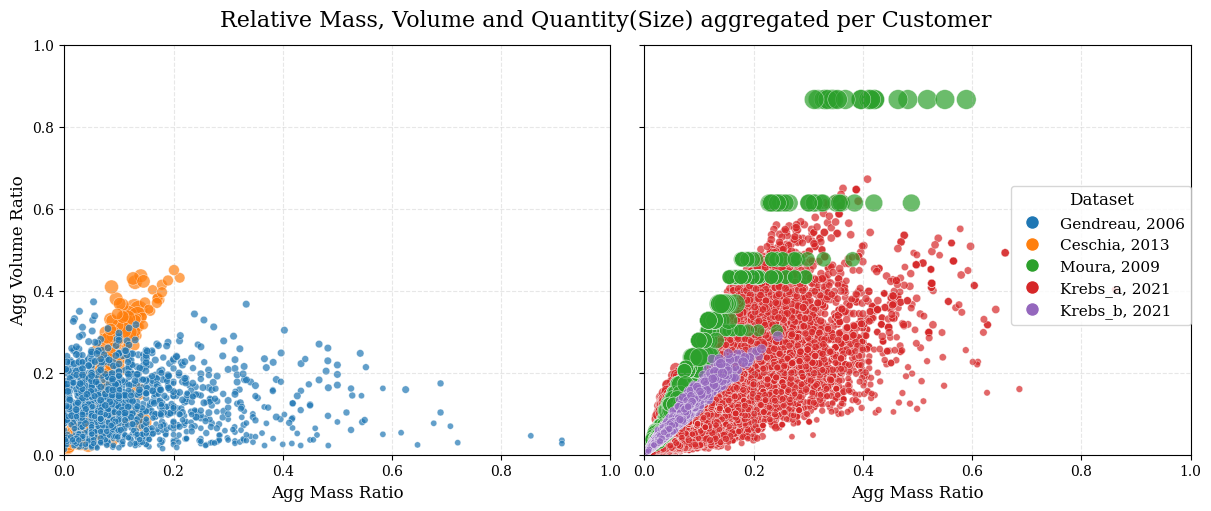
\includegraphics[width=0.85\textwidth]{pictures/comparison_datasets_3lcvrp.png}
    \caption{Comparison aggregated customer demands of different 3L--CVRP/ 3L--VRPTW datasets.}.
    \label{fig:dataset_comparison}
\end{figure}

The dispersion of the data points reflects the diversity of individual instances in terms of volume
and mass dependency. A more balanced profile suggests that some customers tend to order items that
are either mass- or volume-intensive, which supports training the model on more heterogeneous data.
Therefore, the dataset should cover a wide range of cases, varying in mass, volume, and item
quantity per customer. The widest spread is observed in \krebsADataSetText and \gendreauDataSetText datasets serving
both as good dataset candidates for training a classifier. In the overall comparison the \krebsADataSetText dataset
is selected as the most suitable and the properties of this dataset will be further investigated.
The dataset \krebsADataSetText contains 18 different instance types resulting from the combinations
of number of customers, item tyes and items. The following Figure~\ref{fig:krebs_dataset_analysis_detailes} plots
the relative mass and volume of all items requested by individual customers for each of the 18 instances.

\begin{figure}[ht]
    \centering
    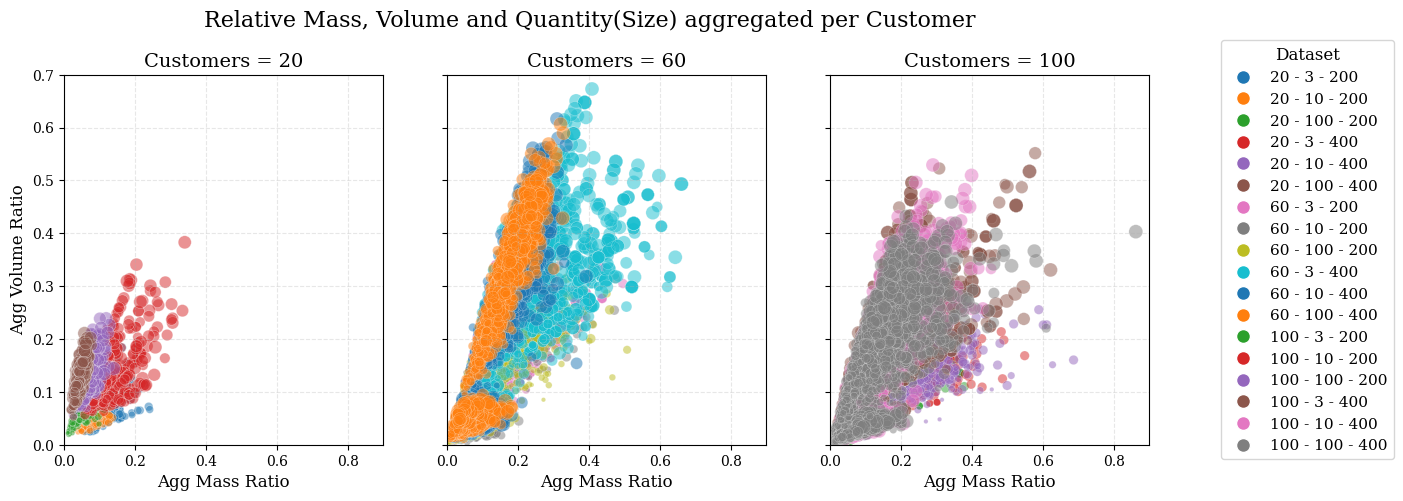
\includegraphics[width=0.85\textwidth]{pictures/krebs_instances_detailed.png}
    \caption[Visualization of different instances of \textcite{krebs_advanced_2021} dataset.]{Visualization of different instances of \krebsADataSetText dataset.}.
    \label{fig:krebs_dataset_analysis_detailes}
\end{figure}

Several insights can be obtained from the analysis of this plot. Firstly, the aggregated relative
volume and mass per customer is significantly lower than for the instances with 60 or 100 customers. Secondly,
the distribution differs from each instance type, ranging from quite linear distributions in a narrow
interval to quite broad distributions.  These two observations need to be considered, when selecting
instances to generate training data for the classifier to avoid a homogenous training set, and
as a consequence poor classifying results with a low accuracy.




%\section{Overview of Public Datasets}
%\section{Evaluation Criteria: Diversity, Realism, Labeling, Size}
%\section{Comparison of Selected Datasets}
%\section{Justification for Dataset Selection}

\begin{comment}
The \gendreauDataSetText dataset contains the relative heaviest items, whereas the other datasets with the exception of
\krebsADataSetText contains lightweight items. The quanitity of ordered items per customer differs the most between
the \gendreauDataSetText and the \mouraDataSetText datasets, and represents the most lowest and the highest values
respectively.
\end{comment}
\chapter{Conclusion and Outlook}
\label{sec:conclusion}
\begin{comment}
The variety of \gls{CLP} applications in logistics is wide, and the urge to consider practical constraints
and realistic datasets is high. For practitioners, heuristics are the first choice as good solutions
can be retrieved in satisfactory time. Exact solutions help to understand the structure of optimal solutions
and to evalutate and enhance existing heuristics. To accelerate exact methods different \gls{ML} enhancements
were presented and the \gls{3L-CVRP} was identified as a promising future use case for \gls{ML} classifiers.
The importance of realistic constraints of the \gls{CLP} were higlighted and the challenges faced when
training the classifier with such constraints were discussed. A dataset from \citeauthor*{krebs_advanced_2021} was identified
was selected for future training of a classifier. To train a \gls{3L-CVRP} classifier that incorporates practical constraints, several next steps are
required. First, a training dataset must be created, consisting of individual tours that are pre-labeled
as feasible or infeasible using an exact \gls{CP} approach. In subsequent training iterations and epochs,
relevant features for accurately predicting feasibility must be evaluated. This includes assessing how
challenging it is to encode each individual constraint as a feature. Once the classifier achieves a
satisfactory level of accuracy, it can be integrated into a complete \gls{3L-CVRP} algorithm. The
classifier will then be used to predict the feasibility of solutions, enabling a comparison between
algorithmic performance with and without the classifier. Finally, the model can be tested on additional
problem instances—such as those introduced in Chapter 5—to evaluate its generalization capabilities.
This will allow the creation of meaningful benchmarks across multiple datasets.
\end{comment}
The wide range of \gls{CLP} applications in logistics underscores the growing need to incorporate practical
constraints and realistic datasets. While heuristics remain the preferred choice for practitioners due to
their efficiency in producing good solutions within acceptable time frames, exact methods play a crucial
role in understanding the structure of optimal solutions and benchmarking heuristics.
To enhance exact approaches, various \gls{ML}-based examples have been presented, and the \gls{3L-CVRP}
has emerged as a promising candidate for the application of machine learning classifiers. This work
emphasized the importance of realistic constraints within the \gls{CLP} context and explored the challenges
of training classifiers under such conditions. A dataset from \citeauthor*{krebs_advanced_2021} was
identified as a suitable foundation for developing a classifier. The next steps involve creating a labeled
training dataset, where individual tours are classified as feasible or infeasible using an exact \gls{CP}
method. Through iterative training and feature evaluation, the goal is to determine which constraints can
be effectively represented and how they impact classification performance. Once a satisfactory level of
accuracy is achieved, the classifier can be integrated into a full \gls{3L-CVRP} algorithm to predict
feasibility and improve decision-making. Finally, the classifier will be tested on additional problem
instances—such as those presented in Chapter 5—to assess its generalizability. This will support the
development of meaningful benchmarks across diverse datasets and contribute to the advancement of
constraint-aware learning in combinatorial logistics problems.


%####################### Appendix #########################
%%############################# Anhang #################################
%\appendix
%\chapter{Mathematischer Anhang}
%\chapter{Programmcodes}

\clearpage
%####################### Literaturverzeichnis #########################
\addcontentsline{toc}{chapter}{\bibname}
\printbibliography
%####################### Selbständigkeitserklärung ####################

\newConfirmationEnglish{Dresden}

%####################### Platzhalter - Abkürzungsverzeichnis muss erstellt werden####################

%\printacronyms[style=bwlimsuper]

%####################### End of Document ####################
\end{document}